\section{Our Approach}

Without loss of generality, for each time step, we partition the volume data into a regular grid of blocks. We then distribute the data blocks among processors, and each processor is assigned to one block.\footnote{Our method can be easily extended to the case that each processor is assigned to multiple data blocks.} In general, a feature can be any interesting object, structure or pattern that is considered relevant for investigation. Here, a feature is defined as the collection of voxels encompassed by a certain iso-surface. Given a sufficient fine grained partitioning, some features can cross multiple data blocks.

We consider the following three factors in our communication scheme design for better performance and scalability:

\begin{itemize}
  \item $N_{com}$ : The number of communications required to build the connectivity information;
  \item $N_{proc/com}$ : The number of processors involved in each communication;
  %\item $N_{data/com}$ : The amount of data involved in each message exchange. 
\end{itemize} 

%In the following sections, we give a detailed description on how to create and maintain such connectivity information using tree structures and then merge them into an undirected unweighted graph to minimize the cost over the above three factors.

\subsection{Extracting Partial Local Features}

%------------------------------------------------
\begin{figure}[t]
	\centering
	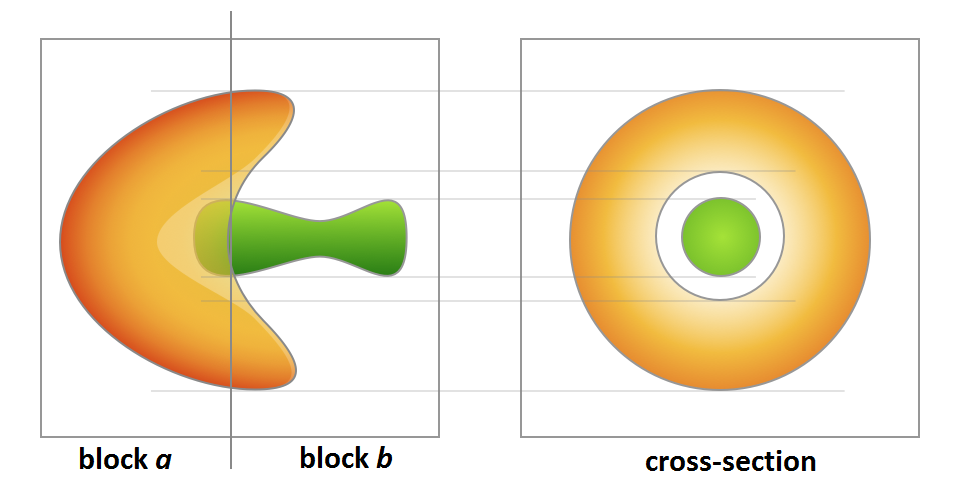
\includegraphics[width=0.9\linewidth]{figure1@2x.png}
	\caption{Two features cross two blocks and share the same centroid on the cross-section.}
	\label{fig:special}
\end{figure}
%------------------------------------------------

Volume features can be extracted using conventional techniques such as region growing, geometry or topology based clustering, or other domain specific algorithms. In this work, we use a standard region-growing algorithm
%\cite{Huang2003}
\cite{Lohmann1998} to identify partial features in each data block. This is done by first spreading a set of seeding points inside each data block, and then grow voxels into separate regions, each regarded as a single feature. As data is distributed, a feature can cross multiple blocks, and each processor is not aware of the partial features identified on the other processors in this stage. 

\subsection{Matching Partial Local Features}

For a feature across multiple blocks, we note that its cross-section in both sides of the adjacent blocks should match. Therefore, we can connect the separate parts of a feature by comparing their cross-sections on the corresponding boundary surfaces. In this case, conceptually, two adjacent processors can find possible matches of partial features though exchanging and comparing their boundary voxels. A ghost area that stores boundary surface belonging to a neighbor may help achieve voxel-wise matching for partial features. However, maintaining such ghost areas requires frequent inter-process communication and is considerably expensive for interactive applications. 

To reduce communication cost and accelerate comparison, we use a simplified method to detect matches. We first represent the cross-section of a feature on a boundary surface as:

\begin{itemize}

\item $P_{centroid}$: The geometric centroid of the cross-section of the feature;

\item $P_{min}$ and $P_{max}$: The minimal and maximal coordinates of the cross-section area.

\end{itemize}

%------------------------------------------------
\begin{algorithm}[t]
\caption{Match of two partial features $f$ and $f^{'}$}
	\begin{algorithmic}
		\IF{$abs(P_{centroid} - P_{centroid}^{'}) \leq 1$ 
		\textbf{and} $abs(P_{min} - P_{min}^{'}) \leq 1$ 
		\textbf{and} $abs(P_{max} - P_{max}^{'}) \leq 1$}
			\STATE return $f$ \textbf{matches} $f^{'}$
		\ENDIF
	\end{algorithmic}
\label{alg:match}
\end{algorithm}
%------------------------------------------------

For two partial features, we then compare their geometric centroids. If the difference is larger that a 1-voxel offset, we consider that they belong to different features. However, only considering geometric centroids is not sufficient to match two features. In some special cases, two different features can have a same geometric centroid on the boundary surface, as shown in Figure~\ref{fig:special}. Therefore, we also need to consider the min-max coordinates of the cross-section areas to detect bipartite matching of partial features, as shown in Algorithm~\ref{alg:match}. In this way, we only need to exchange 3 coordinate values that are sufficient to detect feature connection across a boundary in practice.

\subsection{Creating Local Connectivity Tree}

Based on our method to match the partial local features, we can abstract the local connectivity information using a tree structure as shown in Figure~\ref{fig:match}. Each data block has six direct neighbors (the outermost blocks have less), each with a shared boundary surface. The connectivity tree is constructed taking the block as root, its six adjacent blocks as its first level child nodes, and a leaf is appended to a first level node if a local feature touches the corresponding boundary surface. We note that a feature can touch multiple boundary surfaces and thus be attached to multiple first level nodes.

Note that each voxel in the local data block has a unique global index, and thus each leaf can be encoded using 3 integers (global index for $P_{centroid}$, $P_{min}$ and $P_{max}$). We use $P_{centroid}$ as the feature index, and sort the sibling leaves according to the indexes in ascending order. On the other hand, the root and the first level child nodes can be encoded with the index of corresponding data blocks, which is irrelevant to the number of features-on-boundary (henceforth referred as $N_{fb}$). Therefore, the overall spatial complexity of a local connectivity tree for each data block is $\theta(3*N_{fb})$, which is typically neglectable compared to the volume size. 
%\textcolor{red}{Consider an extreme case that there are 10 thousand features touching each side of the boundary surface, the total memory needed for the local connectivity tree is less than 1MB, neglectable comparing to the volume size itself.}

%------------------------------------------------
\begin{figure}[t]
	\centering
	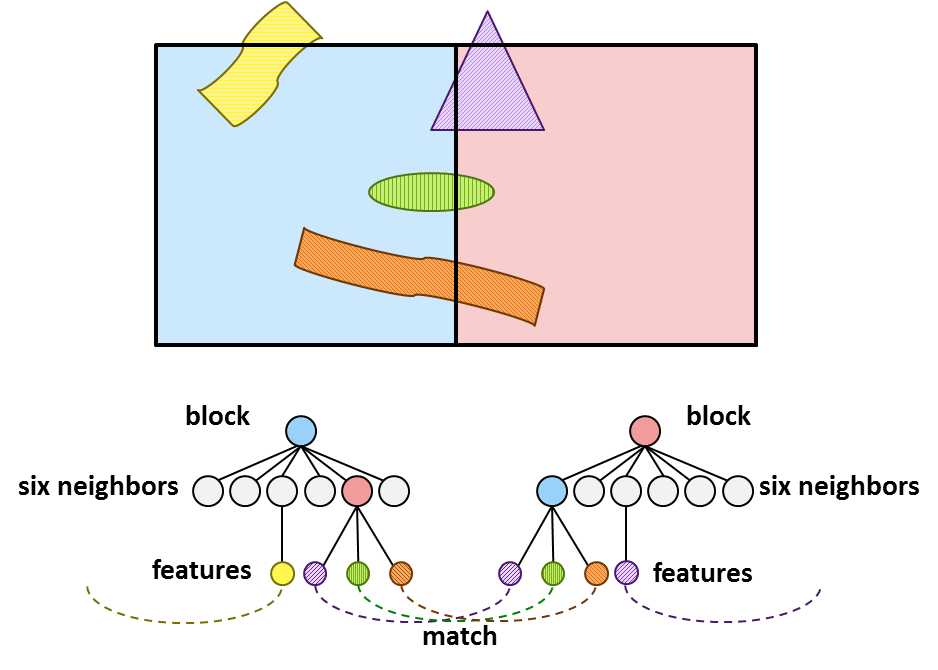
\includegraphics[width=1\linewidth]{match.png}
	\caption{The tree structure used for maintaining local connectivity information, where the root node is encoded with the current block index, its child nodes are encoded with the indexes of its neighboring blocks, and the leaves of each first level child node represent the local partial features. The leaves should match the ones residing on the corespondent neighboring block.}
	\label{fig:match}
\end{figure}
%------------------------------------------------

From the perspective of temporal complexity, the creation of a local connectivity tree does not introduce extra computational cost as it can be done along with the region growing process. The values of $P_{centroid}$, $P_{min}$ and $P_{max}$ are updated only if a feature reaches the boundary surface.
%, and thus the temporal complexity for creating a local connectivity tree remains ${O(\sqrt[2/3]{N_{vexol}})}$, a magnitude less than \textcolor{red}{$O(extraction)$.}

% Algorithm~\ref{alg:local} shows the detailed algorithm of creating local connectivity tree in the region growing process.
% %------------------------------------------------
% \begin{algorithm}
% \caption{Creating Local Connectivity Tree}
% \label{alg:local}
% 
% \begin{algorithmic}
% 	\IF{$t = t_0$}
% 		\STATE $seeds \leftarrow randomVortices()$
% 		\FOR {each $seed$ in $seeds$}
% 			\STATE $feature \leftarrow expendRegion()$
% 			\STATE append $feature$ to $featureList$
% 		\ENDFOR	
% 	\ELSE
% 		\FOR {each $feature$ in $featureList$}
% 			\STATE $feature \leftarrow predictRegion()$
% 			\STATE $feature,P_{centroid},P_{min-max} \leftarrow \textbf{adjustRegion()}$
% 			
% 			\STATE $leaf \leftarrow LEAF(P_{centroid}, P_{min-max})$
% 			\STATE append $leaf$ to $connectivityTree$
% 		\ENDFOR
% 	\ENDIF
% \end{algorithmic}
% 
% \begin{algorithmic} \STATE \end{algorithmic}	% line separator
% 
% \begin{algorithmic}
% \STATE $\textbf{adjustRegion:}$
% 	\IF{Voxel $v$ on boundary surface}
% 		\STATE $P_{centroid} \leftarrow updateBoundaryCentroid()$
% 		\STATE $P_{min-max} \leftarrow updateMinMaxBoundary()$
% 	\ENDIF
% \end{algorithmic}
% \end{algorithm}
% %------------------------------------------------

\subsection{Creating Global Connectivity Information}

After a local connectivity tree being created within each data block, their leaves need to be exchanged and merged to obtain the overall description of a partitioned feature. The exchanging and merging process is decisive in that its effectiveness largely affects the overall performance and scalability of the feature tracking algorithm as a whole.

Based on our application requirements, we represent the global connectivity information into a feature table. Each feature has a global unique ID. The table is indexed by the feature IDs, and each entry lists the processors that contains the corresponding partial local features. Given this simple representation, once a user selects a feature, each related processor can query the table to identify the other processors that need to be communicated to collectively operate on the selected feature.

%In this subsection, we start with a naive solution and discuss progressively through different data exchanging strategy for different scenarios.

% \subsubsection{The Naive Solution}
% 
% A naive solution to obtaining global connectivity information for each feature-on-boundary is to exchange its corresponding leaf with its targeting block. Recall that the first level child nodes are encoded as the ranks of adjacent blocks, and the leaves the global index of the geometric centroid and the min-max boundary on the shared boundary surface. Therefore if a leaf received from neighboring data block matches a local leaf, the two leaves, that is, the two partial features they represented, must share the same boundary section with the same centroid and section region. In other word, these two partial features are resulted by partitioning a original feature, and should be considered as the same feature.
% 
% To prevent a leaf from being resending to the same neighboring block multiple times, it is marked as sent and unless the same feature was found partially reside in another neighboring block, this leaf will be ignored in the next communication to reduce $N_{data/com}$.
% 
% Algorithm~\ref{alg:merge} shows the detailed process to merge matched leaves.
% %------------------------------------------------
% \begin{algorithm}
% \caption{Merging Matched Leaves}
% \label{alg:merge}
% \begin{algorithmic}
% \STATE traverse local connectivity tree in preorder
% \FOR {each $f_{local}$ in $localLeaves$}
% 	\IF{$f_{local}$ is sent = false}
% 		\STATE send $f_{local}$ to targeting block
% 	\ENDIF
% 	\STATE mark $f_{local}$ as sent
% \ENDFOR
% \FOR {each $f_{recv}$ in $recievedLeaves$}
% 	\FOR {each $f_{local}$ in $localLeaves$}
% 		\IF{$f_{recv}$ \textbf{matches} $f_{local}$}
% 			\STATE $f_{local}.id = min(f_{recv}.id, f_{local}.id)$
% 			\STATE mark $f_{local}$ as not sent
% 		\ENDIF
% 	\ENDFOR	
% \ENDFOR
% \end{algorithmic}
% \end{algorithm}
% %------------------------------------------------
% 
% The naive solution may work for data sets with feature-on-boundary that span only a few number of blocks. However, if there exists long curly features partitioned evenly over the data block grid, each block needs to consecutively communicate with its neighbors to incrementally gather and merge a global feature. This requires O(${N_p}$) communications to connect a single feature, where ${N_p}$ is the number of processors in the grid. Consequently, the total communication cost is O(${N_{fb} \times N_p}$) times communication. In addition, since one processor cannot predict how many leaves it will receive from its adjacent processors, it is hard to schedule the communication process.
% 
% %------------------------------------------------
% % \begin{figure*}[ht]
% %   \centering
% %     \subfigure[Local connectivity tree]{
% %       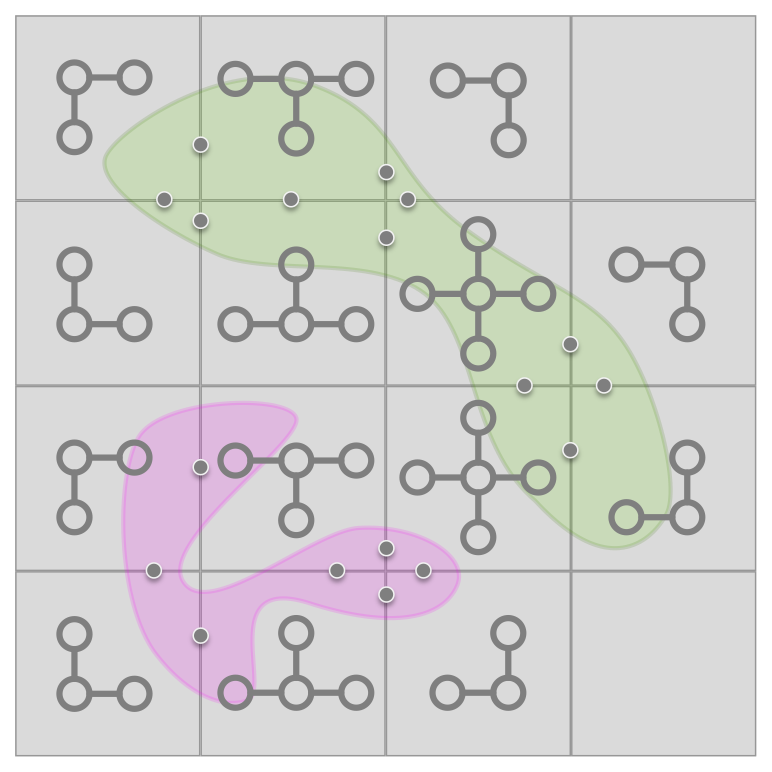
\includegraphics[width=0.23\linewidth]{create.png}
% %       \label{fig:create}
% %     }
% %     \subfigure[Centralized merge with host]{
% %       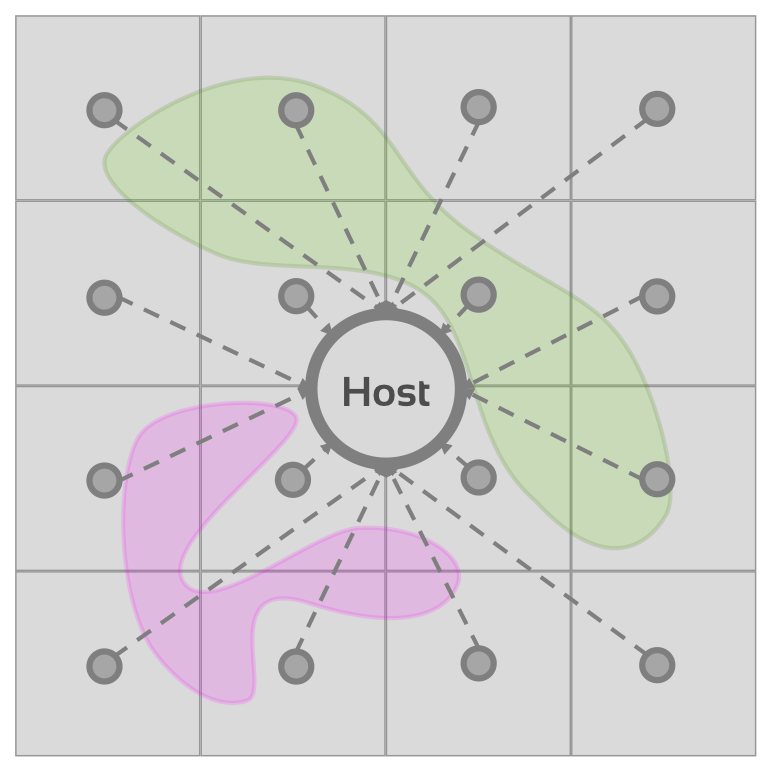
\includegraphics[width=0.23\linewidth]{host.png}
% %       \label{fig:host}
% %     }
% %     \subfigure[Centralized merge without host]{
% %       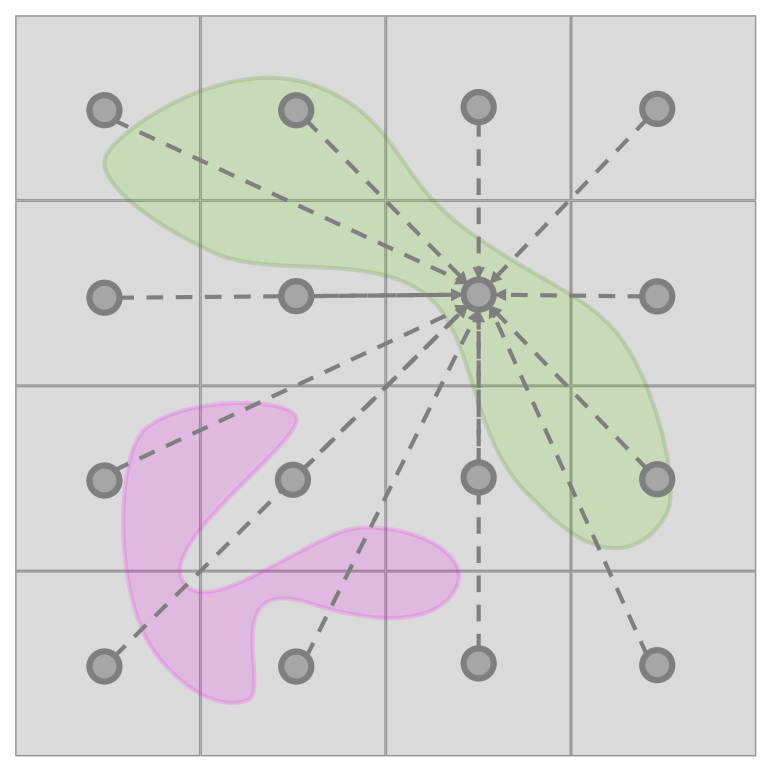
\includegraphics[width=0.23\linewidth]{centralized.png}
% %       \label{fig:centralized}
% %     }
% %     \subfigure[Decentralized merge]{
% %       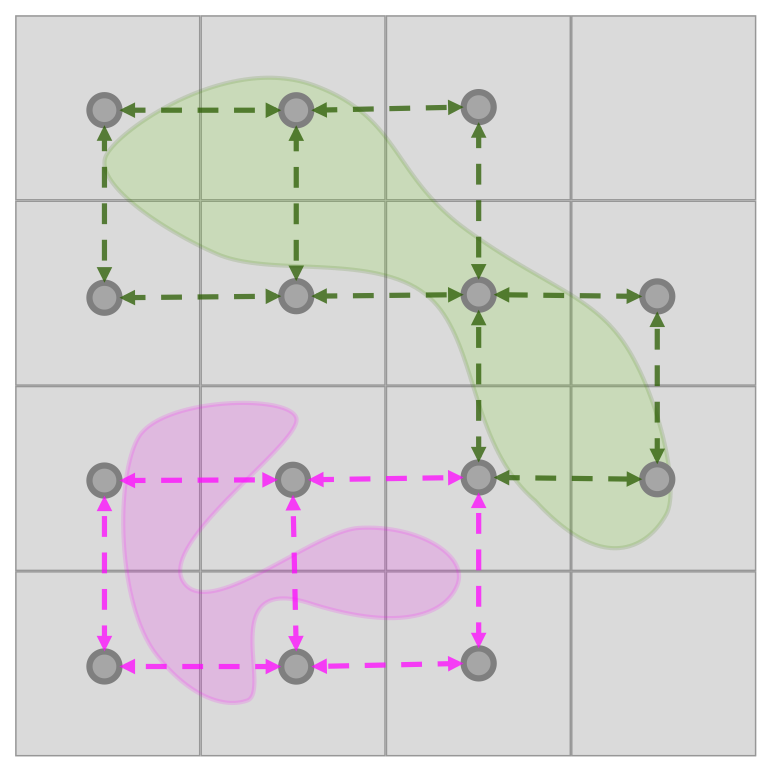
\includegraphics[width=0.23\linewidth]{decentralized.png}
% %       \label{fig:decentralized}
% %     }
% %   \caption[Optional caption for list of figures]{Caption of subfigures \subref{fig:create}, \subref{fig:centralized} and \subref{fig:decentralized}}
% % \end{figure*}
% %------------------------------------------------

\subsubsection{The Centralized Approach}

%One possible solution to improve the aforementioned \textcolor{red}{serialized} approach is to introduce master-slave hierarchy to reduce the number of communication required for merging all leaves. The master-slave hierarchy can be constructed using a separate host processor. 

One possible solution to build the global feature table is to directly use the master-slave paradigm. When the feature extraction process is done, all local connectivity trees are gathered to the host processor. Then the host starts to merge the leaves from each connectivity tree and match the partial features to build the global feature table.

The merit of this centralized approach lies in that it requires inter-processor communication only once, that is, $N_{com} = 1$ for each processor. Moreover, the global feature table can be preserved in the host that it can response to feature queries directly without collecting information from the slaves again. However, this approach has an obvious drawback. Since all local connectivity trees are sent to the host, the number of processors involved in each communication is $N_{proc/com} = N_p$, and there exists potential contention, both in communication and computation, on the host.

\subsubsection{The Decentralized Approach}
\label{sec:decentralized}

A better solution is to decentralize the gathering and merging process from a single host processor to all processors available. After the feature extraction process is done and so does the creation of local connectivity tree, an \emph{all-gather} process starts to exchange all local connectivity trees among processors. Each processor first collect a full copy of all local trees and merge the leaves to obtain the global feature table. However, this approach does not actually resolve the contention problem since every processor acts like the host and it still needs to gather and merge all local trees. 

%------------------------------------------------
\begin{figure}[t]
	\centering
	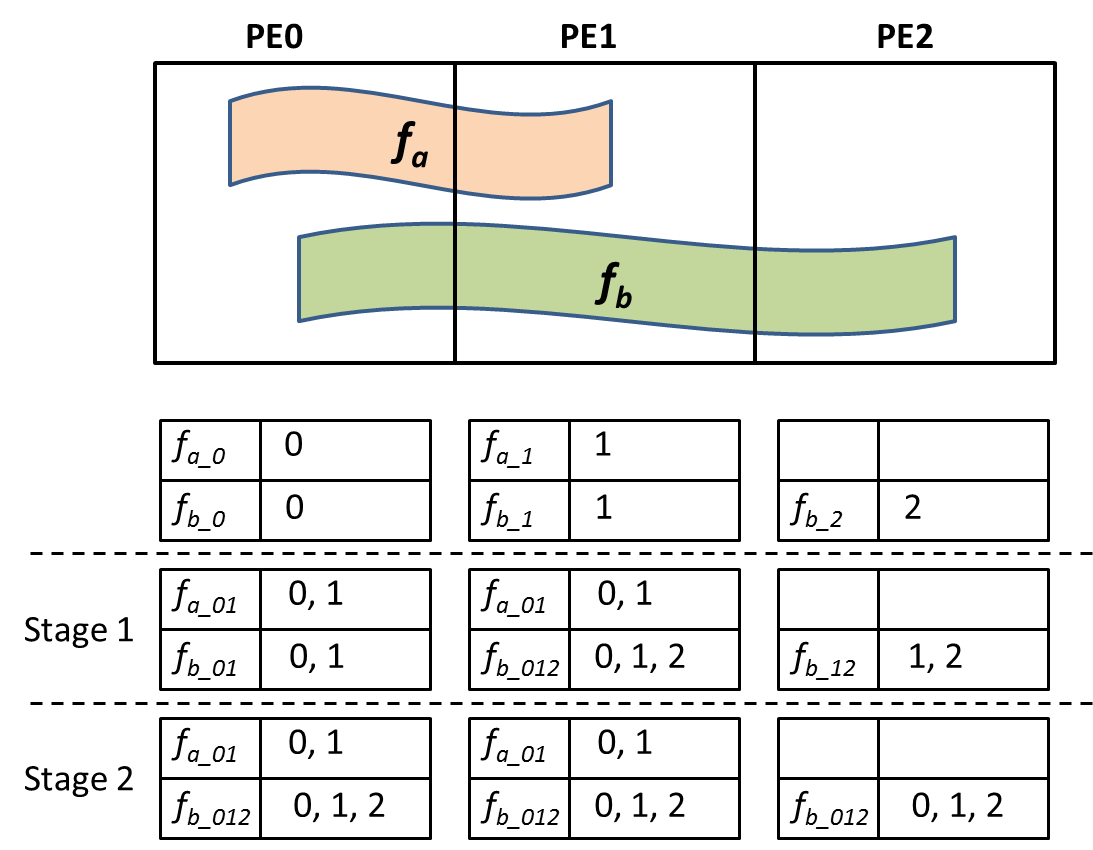
\includegraphics[width=0.9\linewidth]{global_feature_table.png}
	\caption{Construction of partial global feature table with three processors and two features. There are two communication stages. At each stage, each processor only communicates with its immediate neighbors. Each entry of the table is indexed by the feature IDs and lists the processors that contain the corresponding feature.}
	\label{fig:global_table}
\end{figure}
%------------------------------------------------

We observe that, for a real-world data set, it is a rare case that all features span over every data block. In addition, it is unnecessary for each processor to construct a global feature table to contain all features. Each processor only needs to construct a partial table that records the other processors sharing the same set of features. Thus, it is possible for a processor to communicate with a small set of processors to construct the needed portion of the table. However, on the hand, we also observe that each processor has no information of the partial features identified on the other processors. Thus, initially, a processor is not aware of the other processors that can be directly communicated with to gather the partial features. 

Based on these observations, we design an interactive approach that uses multiple stage communication scheme. During each stage, each processor only communicates with its immediate neighbors to exchange and propagate the feature connectivity information. This could be considered as a higher level of region growing process that starts from one seeding block and grows to adjacent blocks by exchanging and merging connectivity information in a bread-first fashion, until all cross-boundary features are connected. 

Figure~\ref{fig:global_table} gives an example of the procedure to construct a partial global feature table with three processors and two features.\footnote{For simplicity, we use an example of 1D partitioning. However, the procedure can be easily extended to 3D cases.} We can see that the feature $f_a$ is identified by the processors PE0 and PE1, and the feature $f_b$ is identified by PE0, PE1 and PE2. Initially, each processor constructs a partial global feature table by only filling the local features with their local IDs, such as $f_{a\_0}$, $f_{b\_2}$, and so on. In the first stage, PE0 exchanges the local connectivity tree with PE1, and PE1 exchanges the tree with PE2. After exchanging trees, each processor independently matches the partial features, and updates the corresponding feature IDs and entries in its table. For example, the ID of $f_a$ has been changed to $f_{a\_01}$ on both PE0 and PE1, and the entry contains the same processor list. However, for $f_b$, as the information has not been propagated between PE0 and PE2, its ID is different on the three processors. In the second stage, each processor still only communicates with its immediate neighbors, and the information of $f_b$ has been propagated to PE0 and PE2 through PE1. Thus the ID and the processor list are all same on the three processors. After an extra communication, each processor detects there not further new information sent from its neighbors, and thus the construction of the partial global feature table is completed.

After having its partial global connectivity table, for any selected features, each processor can easily find the other corresponding processors. For example, in Figure~\ref{fig:global_table}, if $f_a$ is selected, PE0 and PE1 can mutually find that each other belongs to the same communicator, while PE2 is excluded.


% For a regularly partitioned volume data set, there are at most six direct neighbors for each data block. Instead of gathering connectivity information from all non-current data blocks in the grid, we let each data block gather only new leaves from its neighboring blocks within each communication. 
% 
% Figure~\ref{fig:grid2d} gives an example of the process of processor-level region growing in a 2D processor grid.
% 
% %------------------------------------------------
% \begin{figure}[ht]
% 	\centering
% 	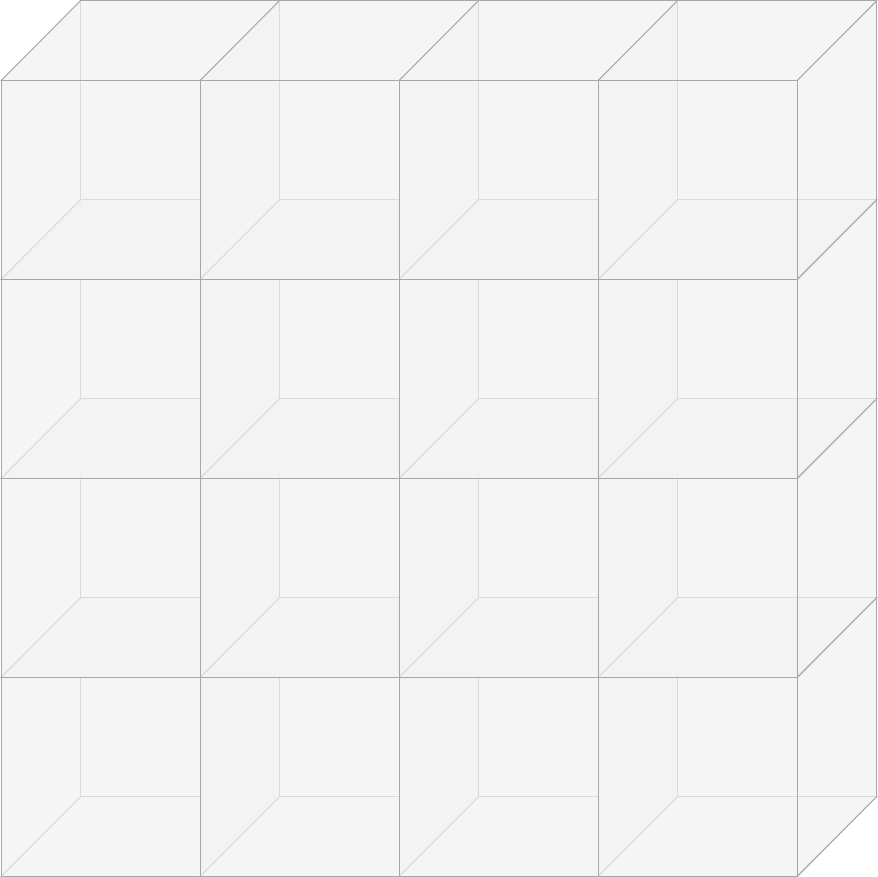
\includegraphics[width=1\linewidth]{grid2d.png}
% 	\caption{The processor-level region growing process in a 2D grid, in which it takes a maximum of 2n-1 times (3n-1 for 3D grid) for the outermost processor to grow to the furthest processor}
% 	\label{fig:grid2d}
% \end{figure}
% %------------------------------------------------

The reason we choose the six-direct-neighbor paradigm is because it can minimize the communication cost. It takes a maximum of ${3n-1}$ times communications, where $n$ denotes the maximum processor number among the axes. This corresponds to the maximum communications needed for propagating the information of a feature that covers the whole domain, although this is nearly impossible in practice. The temporal complexity for garnering all necessary leaves is hence as low as ${O(\sqrt[3]{N_{proc}})}$. And the number of processors involved in each communication is a constant of a maximum of six, $N_{proc/com} \leq 6$.

Another optional paradigm is to let each processor communicate with its 26 neighbors, including the adjacent diagonal blocks. Communication with the adjacent diagonal block takes as much as half the time for any block to reach its furthest diagonal. However, $N_{proc/com}$  is also increased to 26. For data sets where features only span over a small number of blocks, the 6-direct-neighbor paradigm outweighs the 26-neighbors paradigm in communication complexity.

% To schedule the communication within neighboring processors, we use two schedule flags, \emph{toSend} and \emph{toRecv}, to indicate whether a processor need to send or receive information to/from its neighboring processors. Whenever a processor receives information that can be merged into its existing table, we assume the neighboring blocks might receive further connectivity information from their neighbors. In this case, the \emph{toRecv} flag is set to true until the connectivity graph is \textcolor{red}{saturated}; On the other hand, the \emph{toSend} flag is set in accordance to whether one of the neighboring blocks need to receive leaves, which can be obtained by gathering the neighboring \emph{toRecv} flags. Each data block will keep exchanging connectivity information until both \emph{toSend} and \emph{toRecv} flags are set to false.
% 
% The detailed scheduling algorithm is depicted in Algorithm~\ref{alg:schedule}.
% %------------------------------------------------
% \begin{algorithm}
% \caption{Decentralized Local Merge}
% \label{alg:schedule}
% 	\begin{algorithmic}
% 	\STATE $toSend, toRecv \leftarrow true$
% 	\STATE $\delta \leftarrow localLeaves$
% 	\WHILE {$toSend$ is true \textbf{or} $toRecv$ is true}
% 		\STATE $target \leftarrow myRank$ \textbf{if} $toRecv$ = $true$
% 		\STATE $procsToSync \leftarrow gatherNeighbor(target)$
% 		
% 		\FOR {each $proc$ in $procsToSync$}
% 			\IF {$toSend$ = $true$}
% 				\STATE send $\delta$ to $proc$
% 			\ENDIF
% 			\IF {$toRecv$ = $true$}
% 				\STATE receive $\delta\prime$ from $proc$
% 			\ENDIF
% 		\ENDFOR
% 		
% 		\STATE $toSend \leftarrow false$ \textbf{if} $procsToSync$ is empty \textbf{else} $true$
% 		\STATE $toRecv \leftarrow false$ \textbf{if} $\delta$ = $Merge(\delta, \delta\prime)$ \textbf{else} $true$
% 		\STATE $\delta \leftarrow Merge(\delta, \delta\prime)$ \textbf{if} $toRecv$ is true
%   \ENDWHILE
%   \end{algorithmic}
% \end{algorithm}
% %------------------------------------------------

\subsection{Updating Global Connectivity Information}

%------------------------------------------------
\begin{figure}[t]
	\centering
	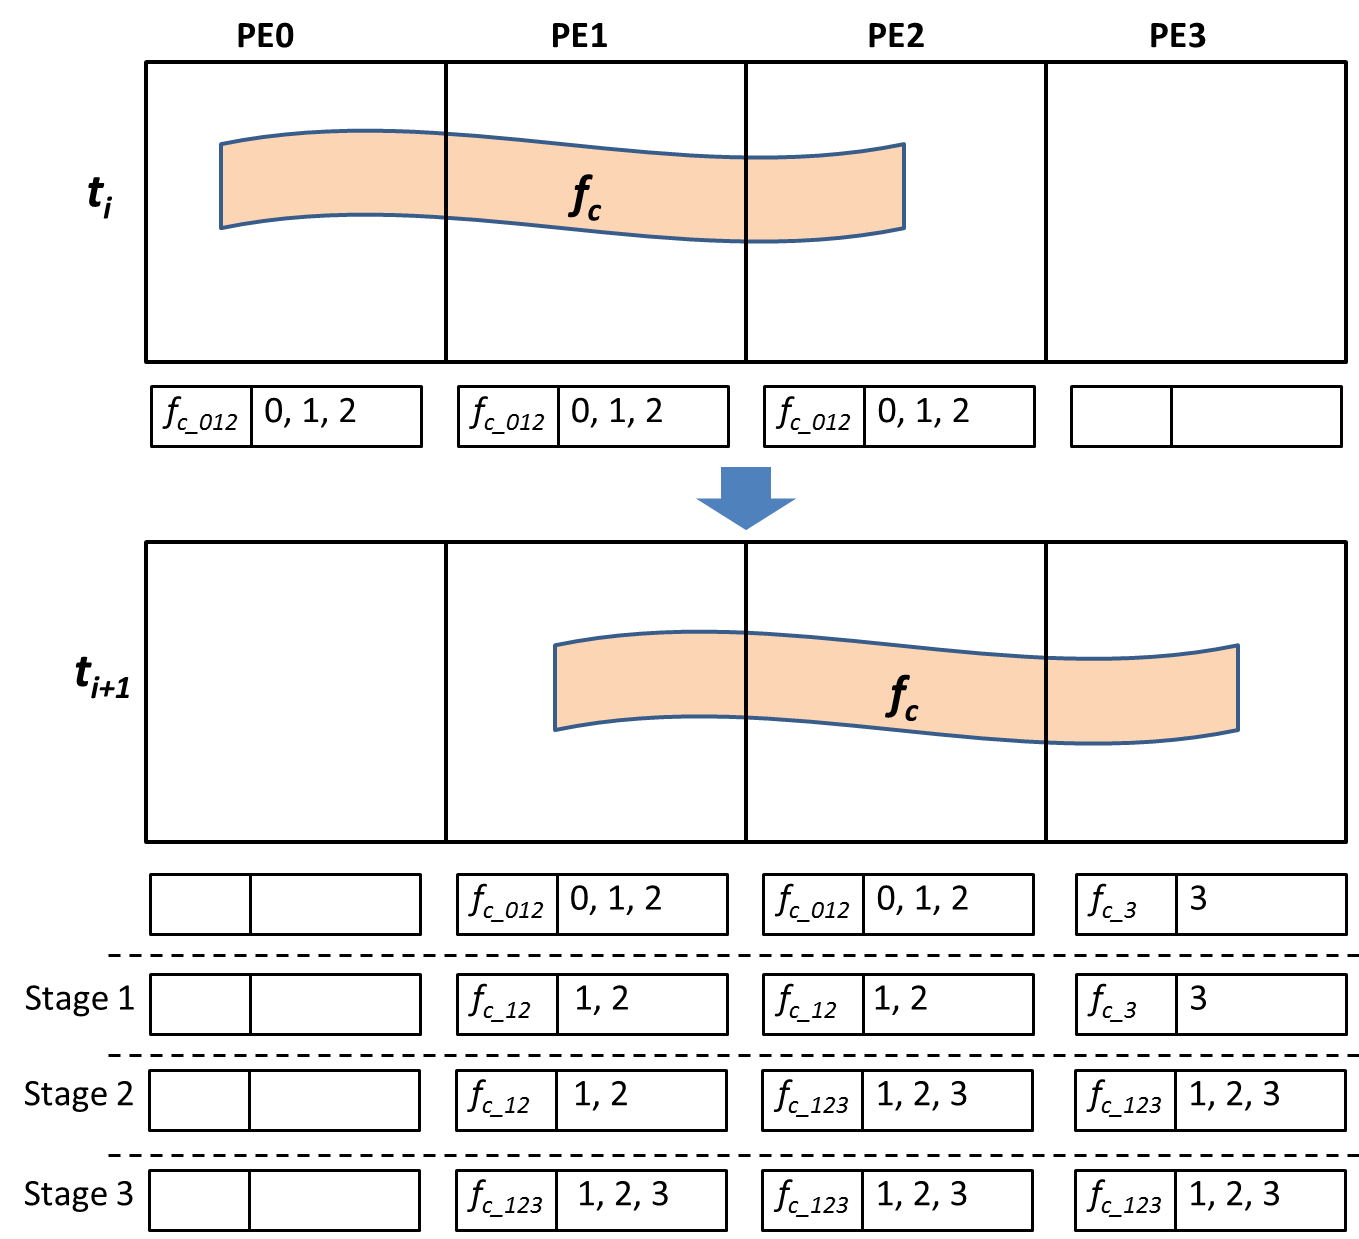
\includegraphics[width=1\linewidth]{global_grow_feature_table.png}
	\caption{Update of partial global feature table with four processors and one feature. There are three communication stages to record the possible shrinking and expanding of the feature. }
	\label{fig:hybrid}
\end{figure}
%------------------------------------------------

To track features, we can construct the global connectivity table for each time step. However, if the time interval is sufficiently small for generating the data, volumetric features may drift but should not change drastically in neither size, shape nor location. We assume that the changes of each feature are within the range of one block. Base on this assumption, we can optimize feature tracking by incrementally updating global connectivity information over time.

As depicted in Figure~\ref{fig:hybrid}, each processor constructs a partial global feature table at a time step $t_i$. Meanwhile, for each feature, we maintain a communicator, $\textbf{C}$, which contains the corresponding processors. For example, the feature, $f_c$, spans over PE0, PE1, and PE2. These three processors have the same table. The table of PE3 is empty at $t_i$. PE0, PE1 and PE2 belong to the same communicator $\textbf{C}$.

For the next time steps, $t_{i+1}$, each processor continues to extract partial local features, and uses overlapping to detect the correspondence of features over time. For the same features, their IDs are retained in the partial global feature table. For the new features, their IDs are added into the table. And the IDs are erased from the table, if the features drift away from the block. As shown in Figure~\ref{fig:hybrid}, $f_c$ leaves PE0 and enters PE3. In this case, the table of PE0 becomes empty, and the table of PE3 adds a new entry. Here, we note that the feature ID on PE3 is not same as the others, as the feature has not been matched yet. In addition, PE0, PE1 and PE2 still belong to $\textbf{C}$. 

Then we start the updating of the connectivity information. In the first stage, PE0, PE1, and PE2 perform an \emph{all-gather} operation within their communicator $\textbf{C}$ to update the connectivity. PE0 is then removed from the corresponding entry on PE1 and PE2, and also removed from $\textbf{C}$. In the second stage, each processor exchanges the local connectivity information with the immediate neighbors as the decentralized approach in Section~\ref{sec:decentralized}. The information of $f_c$ is propagated between PE2 and PE3. In the third stage, all the processors in the communicator $\textbf{C}$ perform an \emph{all-gather} operation again to update the connectivity. PE3 is propagated to the rest of processors $\textbf{C}$, and then PE1, PE2, and PE3 have the same table at $t_{i+1}$. Given the unified information, we can then update the communicator $\textbf{C}$ by including PE3 with respect to $f_c$. 

This update procedure can be easily extended to the circumstances with more processors and features. We note that the cost of collective communication is marginal within a communicator of limited size. By leveraging this nice property, for each feature, we only need at most three stages to update the connectivity information, no matter the length of the feature.  

%If these are no new blocks involved, only two communication stages are sufficient to update the connective information for a shrinking feature. 

%, when the global connectivity graph is obtained, the local communicators will be updated for the next time step, $t_{i+1}$, with the union of processors that share the same set of feature-on-boundary with the current processor. The leaves from these data blocks are necessary to complete the global connectivity graph no matter which gathering approach is used. Hence, for these must-involve data blocks, we apply the all-gather-decentralize approach, allowing the minimum one-time synchronization to finish gathering all leaves that are necessary for updating the connectivity graph based on the graph created at the previous time step $t$. Then, processor-level region growing, a.k.a the processor-level-decentralize approach is applied to extend the boundary of data blocks, obtaining newly connected blocks caused by the evolution of the volume data. Again, only those leaves that are changed and not yet sent will be exchanged. This ensure that we minimize the amount of data being sent over network.

% further optimizing the aforementioned decentralized-local-merge approach. Utilizing the prediction-correction approach for single processor feature tracking we can further reduces the communication cost required to complete the whole connectivity graph.
% 
% As depicted in as depicted in Figure~\ref{fig:hybrid}, for every time step $t_i$, when the global connectivity graph is obtained, the local communicators will be updated for the next time step, $t_{i+1}$, with the union of processors that share the same set of feature-on-boundary with the current processor. The leaves from these data blocks are necessary to complete the global connectivity graph no matter which gathering approach is used. Hence, for these must-involve data blocks, we apply the all-gather-decentralize approach, allowing the minimum one-time synchronization to finish gathering all leaves that are necessary for updating the connectivity graph based on the graph created at the previous time step $t$. Then, processor-level region growing, a.k.a the processor-level-decentralize approach is applied to extend the boundary of data blocks, obtaining newly connected blocks caused by the evolution of the volume data. Again, only those leaves that are changed and not yet sent will be exchanged. This ensure that we minimize the amount of data being sent over network.
% 
% The detail algorithm of the hybrid approach is given in Algorithm~\ref{alg:hybrid}.
% %------------------------------------------------
% \begin{algorithm}
% \caption{Prediction-enabled Local Merge}
% \label{alg:hybrid}
% 	\begin{algorithmic}
% 		\STATE Let $P_{f_i} \equiv$ all processors that contains feature $f_i$
% 		\IF{$t = t_0$}
% 			\STATE $localCom \leftarrow union(P_{f_i})$ for all $f_i$ in current data block
% 		\ELSE
% 			\FOR {each $proc$ on boundary of $localCom$ \textbf{do}}
% 				\STATE $P_{f_i}^{'} \leftarrow decentralizedLocalMerge(proc)$
% 			\ENDFOR
% 			\STATE $localCom \leftarrow union(P_{f_i}^{'})$
% 		\ENDIF
% 	\end{algorithmic}
% \end{algorithm}
% %------------------------------------------------ 


%
% After specific features have been identified from a single time step, we track their evolution over time using the prediction-correction approach~\cite{Muelder2009}. Given a sufficiently small temporal interval, feature locations are consistent for consecutive time step. The location of a feature at a time step is predicted and refined using the location(s) of the feature in previous time step.
%Once the prediction is made, the actual region can be obtained by adjusting the surface of the predicted region: First shrink the edge surface points to obtain the mutual region between consecutive time steps, and then use of a region-growing method to generate the refined region, as depicted in Figure~\ref{fig:predict-correct}. 

% Both the region-growing and prediction-correction approaches were proven effective and efficient for tracking feature on a single processor%\cite{Muelder2009}.
% However, when the size of the volume becomes too large to be fitted into a single processor, a cluster of processors is often needed to process the data in parallel. One challenge of parallelization lies in that it can be difficult to obtain the global feature descriptions unless they can be shared and merged in an efficient way. This is because the features may span over multiple processors and partial features in different data blocks are operated independently. An intuitive way of exchanging such feature information is to first find how features span over multiple processors, and then merge them according to the connectivity information.

% %------------------------------------------------
% \begin{figure}[ht]
% 	\centering
% 	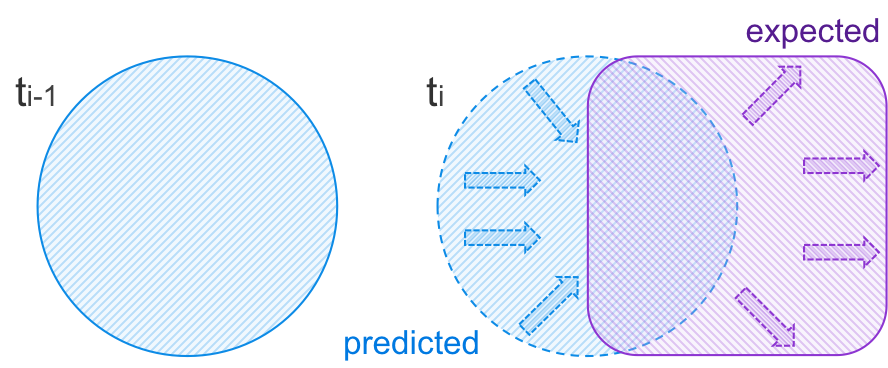
\includegraphics[width=0.9\linewidth]{predict_correct.png}
% 	\caption{The predict-correct feature tracking approach. First the predicted region is derived using location(s) of that feature in previous time step $t_{i-1}$. Then we shrink the portion that does not satisfy the criteria in $t_i$, which obtain us the mutual portion of that in $t_{i-1}$ and $t_i$. Finally we apply region growing again to obtain the expected feature region depicted.}
% 	\label{fig:predict-correct}
% \end{figure}
% %------------------------------------------------